\documentclass[aspectratio=169,10pt]{beamer}

\usetheme{Madrid}
\usecolortheme{seahorse}
\useinnertheme{circles}
\useoutertheme{miniframes}

\usepackage[utf8]{inputenc}
\usepackage{graphicx}
\usepackage{booktabs}
\usepackage{array}
\usepackage{colortbl}
\usepackage{xcolor}
\usepackage{amsmath}
\usepackage{caption}

\graphicspath{%
  {./}%
  {../plots/}%
  {../plots/inventory/}%
  {../plots/suite31/}%
  {../plots/suite32/}%
  {../plots/suite33/}%
  {../plots/resampling/}%
  {../results/final/modality_tables/}%
  {../results/final/modality_tables_optimized/}%
  {../results/final/combined_best/}%
  {../results/final/final_pipeline/}%
}

\setbeamertemplate{caption}[numbered]
\setbeamercovered{transparent}

\title[AI4Pain 2026]{AI4Pain 2026 Challenge \\ NoPain / PainArm / PainHand Recognition}
\subtitle{Two-Stage Physiological Pipeline}
\author{Soyeb Pervez Jim}
\institute{Department of EEE, University of Dhaka}
\date{\today}

\begin{document}

\begin{frame}
  \titlepage
\end{frame}

\begin{frame}{Outline}
  \tableofcontents
\end{frame}

% ===================================================================
\section{Challenge Overview}
% ===================================================================

\begin{frame}{Challenge Overview}
  \textbf{AI4Pain 2026} — multimodal physiological pain recognition.
  \begin{itemize}
    \item \textbf{Task:} 3-class classification — \texttt{NoPain}, \texttt{PainArm}, \texttt{PainHand}.
    \item \textbf{Modalities:} BVP (blood volume pulse), EDA (electrodermal), Resp (respiration), SpO\textsubscript{2}.
    \item \textbf{Sampling:} 4 channels per segment, 1000--1118 samples (median 1022).
    \item \textbf{Scoring:} macro-F1 / accuracy on held-out validation subjects.
    \item \textbf{Key constraint:} subject-disjoint splits $\Rightarrow$ LOSO evaluation required.
  \end{itemize}
\end{frame}

\begin{frame}{Objectives}
  \begin{enumerate}
    \item Build a reliable 3-class pipeline that \textbf{beats single-modality baselines}.
    \item Decouple \textbf{detection} (NoPain vs Pain) from \textbf{localization} (Arm vs Hand).
    \item Explore \textbf{subject-level normalization} to beat cross-subject variance.
    \item Explore \textbf{resampling} (truncate, linear, polyphase) for variable lengths.
    \item Quantify \textbf{per-modality contribution} at each stage.
    \item Deliver a reproducible \texttt{stage1 + stage2 + decoder} recipe.
  \end{enumerate}
\end{frame}

% ===================================================================
\section{Dataset Analysis}
% ===================================================================

\begin{frame}{Dataset — Shape \& Balance}
  \begin{columns}[T,onlytextwidth]
    \column{0.55\textwidth}
    \begin{itemize}
      \item \textbf{Train:} $(1476, 4, 1000)$ — 41 subjects.
      \item \textbf{Validation:} $(432, 4, 1000)$ — 12 subjects.
      \item No subject overlap between splits.
      \item Every subject: exactly \textbf{12 / 12 / 12} (NoPain / PainArm / PainHand).
      \item Balanced at subject level $\Rightarrow$ enables exact-count decoding.
    \end{itemize}
    \column{0.45\textwidth}
    \centering
    
\includegraphics[width=\linewidth]{subject_class_counts_heatmap.png}
  \end{columns}
\end{frame}

\begin{frame}{Dataset — Segment Lengths \& Integrity}
  \begin{columns}[T,onlytextwidth]
    \column{0.5\textwidth}
    \begin{itemize}
      \item Raw lengths: min 990, median \textbf{1022}, max 1118.
      \item Padding-NaN at tail: 36/1476 per signal (train).
      \item \textbf{No} interior NaN / Inf in any segment.
      \item \textbf{Constant SpO\textsubscript{2}}: 254 train + 95 val segments (flat lines).
      \item SpO\textsubscript{2} has 349 byte-duplicate segments.
      \item Conclusion: SpO\textsubscript{2} is the weakest, most degraded channel.
    \end{itemize}
    \column{0.5\textwidth}
    \centering
    
\includegraphics[width=\linewidth]{segment_lengths_hist.png}
  \end{columns}
\end{frame}

\begin{frame}{Dataset — Signal Ranges}
  \centering
  
\includegraphics[width=0.7\linewidth]{signal_range_boxplots.png}
  \begin{itemize}
    \small
    \item BVP: near-centered, narrow dynamic range.
    \item EDA: 0--19\,$\mu$S, heavy right tail.
    \item Resp: arbitrary units, symmetric around 0.
    \item SpO\textsubscript{2}: 0--100\,\%, dominated by valid 90--100 with occasional zeros.
  \end{itemize}
\end{frame}

% ===================================================================
\section{Baseline}
% ===================================================================

\begin{frame}{Baseline — Paper Modality Accuracies}
  \centering
  \small
  \begin{tabular}{lll}
    \toprule
    \textbf{Set} & \textbf{Modality} & \textbf{Accuracy} \\
    \midrule
    Validation & EDA        & 43.05\,\% \\
    Validation & BVP        & 43.75\,\% \\
    Validation & Resp       & 35.64\,\% \\
    Validation & SpO\textsubscript{2} & 35.87\,\% \\
    Validation & Multimodal & 41.66\,\% \\
    \midrule
    Test & EDA        & -- \\
    Test & BVP        & -- \\
    Test & Resp       & -- \\
    Test & SpO\textsubscript{2} & -- \\
    Test & Multimodal & -- \\
    \bottomrule
  \end{tabular}

  \vspace{6pt}
  \textbf{Takeaway:} paper baseline stuck near chance (33\,\%) for 3-class. Multimodal under-performed single best (BVP). Target: beat 43.75\,\%.
\end{frame}

% ===================================================================
\section{Our Approach}
% ===================================================================

\begin{frame}{Our Approach — Two-Stage Pipeline}
  \begin{block}{Architecture}
    \textbf{Stage 1:} binary NoPain vs Pain detector (BVP+EDA features, XGBoost).\\
    \textbf{Stage 2:} binary PainArm vs PainHand localizer (Resp features, calibrated LogReg).\\
    \textbf{Decoder:} joint-weighted exact-count (12/12/12) over (p1, p2).
  \end{block}
  \begin{itemize}
    \item Stage 1 picks up \textbf{physiological arousal} (cardiovascular + sudomotor).
    \item Stage 2 exploits \textbf{respiration} as the best arm-vs-hand separator.
    \item Decoder enforces the known per-subject class distribution.
  \end{itemize}
\end{frame}

\begin{frame}{Our Approach — Default Best Config}
  \small
  \begin{columns}[T,onlytextwidth]
    \column{0.5\textwidth}
    \textbf{Stage 1}
    \begin{itemize}
      \item resample: \texttt{truncate1022}
      \item norm: \texttt{subject\_robust}
      \item features: \texttt{bvp\_eda\_core} (98)
      \item model: \texttt{xgb}
      \item anchor: \texttt{center}, $\lambda=0.5$
    \end{itemize}
    \column{0.5\textwidth}
    \textbf{Stage 2}
    \begin{itemize}
      \item resample: \texttt{truncate1022}
      \item norm: \texttt{subject\_z}
      \item features: \texttt{resp\_all} (44)
      \item model: \texttt{logreg}, \texttt{robust} scaler
      \item calibration: \texttt{isotonic}
    \end{itemize}
  \end{columns}
  \vspace{4pt}
  \textbf{Combined decoder:} \texttt{joint\_weighted} with $w_0{=}0.8$, $w_1{=}1.2$, $w_2{=}1.4$.
\end{frame}

% ===================================================================
\section{Preprocessing}
% ===================================================================

\begin{frame}{Preprocessing}
  \begin{itemize}
    \item \textbf{Length alignment:} truncate / linear-resample / polyphase-resample to \textbf{1022} samples.
    \item \textbf{Padding handling:} drop tail-NaN before feature extraction.
    \item \textbf{Feature extraction:} 248 features per segment (time, frequency, morphology, Hjorth, entropy).
    \item \textbf{Subject-level normalization:}
      \begin{itemize}
        \item \texttt{subject\_z}: $(x-\mu_s)/\sigma_s$.
        \item \texttt{subject\_robust}: median / IQR per subject.
      \end{itemize}
    \item \textbf{Feature subsets:}
      \texttt{bvp\_eda\_core} (98), \texttt{bvp\_eda\_resp\_small}, \texttt{resp\_all} (44), \texttt{all} (177--212).
    \item \textbf{Finding:} \texttt{1022} beats \texttt{1000}; \texttt{truncate} beats linear/poly resampling overall.
  \end{itemize}
\end{frame}

\begin{frame}{Preprocessing --- Resampling Example}
  \centering
  
\includegraphics[width=0.8\linewidth]{resample_example_train_1_NoPain_1.png}
\end{frame}

% ===================================================================
\section{Post-processing}
% ===================================================================

\begin{frame}{Post-processing}
  \begin{itemize}
    \item \textbf{Probability calibration:}
      \begin{itemize}
        \item Stage 1: \texttt{sigmoid} (Platt).
        \item Stage 2: \texttt{isotonic} — essential for weighted decoding.
      \end{itemize}
    \item \textbf{Anchor refinement (Stage 1):} pull scores toward the subject's \texttt{NoPain} centroid, $\lambda=0.5$ (\texttt{anchor\_center\_l05}).
    \item \textbf{Decoders:}
      \begin{itemize}
        \item \texttt{split\_topk}: top-$k$ per class, known counts.
        \item \texttt{joint\_weighted}: optimal assignment over joint (p1,p2) with class weights — \emph{winner}.
      \end{itemize}
    \item \textbf{Exact-count decoding:} enforces 12 / 12 / 12 per subject on validation.
  \end{itemize}
\end{frame}

% ===================================================================
\section{Per-Stage Metrics}
% ===================================================================

\begin{frame}{Stage 1 --- Best Configs (Validation Macro-F1)}
  \centering
  \scriptsize
  \begin{tabular}{lccccc}
    \toprule
    \textbf{Config} & \textbf{Macro-F1} & \textbf{Acc} & \textbf{Prec NoPain} & \textbf{Rec NoPain} \\
    \midrule
    \rowcolor{yellow!20} truncate1022 $|$ subject\_robust $|$ bvp\_eda\_core $|$ xgb $|$ anchor\_center\_l05 & \textbf{0.833} & \textbf{0.852} & 0.778 & 0.778 \\
    truncate1022 $|$ subject\_robust $|$ bvp\_eda\_core $|$ xgb $|$ base            & 0.828 & 0.847 & 0.771 & 0.771 \\
    poly1022     $|$ subject\_robust $|$ bvp\_eda\_core $|$ xgb $|$ base            & 0.828 & 0.847 & 0.771 & 0.771 \\
    truncate1022 $|$ subject\_robust $|$ bvp\_eda\_core $|$ xgb $|$ anchor\_z\_l05  & 0.828 & 0.847 & 0.771 & 0.771 \\
    truncate1022 $|$ subject\_z      $|$ bvp\_eda\_core $|$ xgb $|$ base            & 0.823 & 0.843 & 0.764 & 0.764 \\
    \midrule
    \textit{RBF SVM best (ref)} & 0.818 & 0.838 & 0.757 & 0.757 \\
    \bottomrule
  \end{tabular}

  \vspace{4pt}
  \textbf{Winner:} XGB on BVP+EDA with subject-robust norm + center anchor, $\lambda=0.5$.
\end{frame}

\begin{frame}{Stage 1 --- Confusion \& Calibration}
  \begin{columns}[T,onlytextwidth]
    \column{0.5\textwidth}
    \centering
    
\includegraphics[width=\linewidth]{suite32/confusion_matrix_1.png}\\
    \tiny Best stage-1 confusion matrix (suite 32).
    \column{0.5\textwidth}
    \centering
    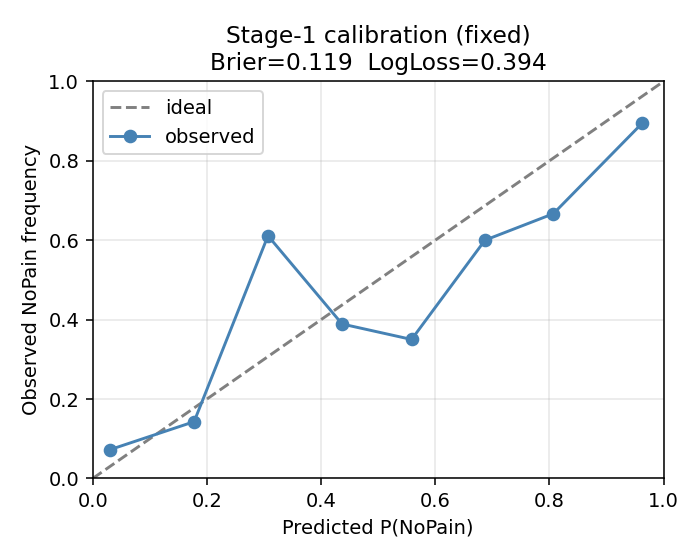
\includegraphics[width=\linewidth]{calibration_stage1_fixed.png}\\
    \tiny Corrected calibration: predicted P(NoPain) vs observed NoPain freq. Brier = 0.119, LogLoss = 0.394, corr = 0.88. \\
    \tiny (Original \texttt{calibration\_best.png} had wrong axis label --- sklearn default \texttt{pos\_label=1} = Pain.)
  \end{columns}
\end{frame}

\begin{frame}{Stage 1 --- Resample $\times$ Feature-set Heatmap}
  \centering
  
\includegraphics[width=0.65\linewidth]{suite32/heatmap_resample_featureset.png}
\end{frame}

\begin{frame}{Stage 2 --- Best Recipe}
  \begin{block}{Winning stage-2 family}
    \texttt{subject\_z} $|$ \texttt{resp\_all} $|$ \texttt{logreg} $|$ \texttt{robust} scaler $|$ \texttt{isotonic} calibration.
  \end{block}
  \begin{itemize}
    \item \textbf{Resp} carries the strongest arm-vs-hand localization signal.
    \item Larger model families (XGB, RF, SVM) did \emph{not} reliably beat calibrated logreg.
    \item Isotonic calibration is \textbf{required} for weighted joint decoding to gain.
    \item Pairwise ranking and latent-intensity splits did not win.
  \end{itemize}
\end{frame}

\begin{frame}{Stage 2 --- Decoder Heatmap}
  \centering
  
\includegraphics[width=0.65\linewidth]{suite31/heatmap_stage2_decoder.png}
\end{frame}

% ===================================================================
\section{Modality Tables}
% ===================================================================

\begin{frame}{Stage 1 --- Modality Table (Overall)}
  \centering
  \small
  \begin{tabular}{lrrr}
    \toprule
    \textbf{Modality} & \textbf{n\_feat} & \textbf{val\_acc} & \textbf{val\_auc} \\
    \midrule
    BVP          & 52  & 0.806 & 0.858 \\
    EDA          & 46  & 0.755 & 0.829 \\
    RESP         & 44  & 0.606 & 0.580 \\
    SpO\textsubscript{2} & 35  & 0.657 & 0.642 \\
    \rowcolor{green!15} EDA+BVP      & 98  & \textbf{0.829} & \textbf{0.904} \\
    EDA+BVP+RESP & 142 & 0.810 & 0.900 \\
    All          & 177 & 0.819 & 0.905 \\
    \bottomrule
  \end{tabular}
\end{frame}

\begin{frame}{Stage 1 --- Modality Classwise}
  \centering
  \scriptsize
  \begin{tabular}{lrrrrrr}
    \toprule
    \textbf{Modality} & \textbf{NoPain P} & \textbf{Pain P} & \textbf{NoPain R} & \textbf{Pain R} & \textbf{NoPain F1} & \textbf{Pain F1} \\
    \midrule
    BVP          & 0.708 & 0.854 & 0.708 & 0.854 & 0.708 & 0.854 \\
    EDA          & 0.632 & 0.816 & 0.632 & 0.816 & 0.632 & 0.816 \\
    RESP         & 0.410 & 0.705 & 0.410 & 0.705 & 0.410 & 0.705 \\
    SpO\textsubscript{2} & 0.486 & 0.743 & 0.486 & 0.743 & 0.486 & 0.743 \\
    \rowcolor{green!15} EDA+BVP      & \textbf{0.743} & \textbf{0.872} & 0.743 & 0.872 & 0.743 & 0.872 \\
    EDA+BVP+RESP & 0.715 & 0.858 & 0.715 & 0.858 & 0.715 & 0.858 \\
    All          & 0.729 & 0.865 & 0.729 & 0.865 & 0.729 & 0.865 \\
    \bottomrule
  \end{tabular}
\end{frame}

\begin{frame}{Stage 2 --- Modality Table (Overall)}
  \centering
  \small
  \begin{tabular}{lrrr}
    \toprule
    \textbf{Modality} & \textbf{n\_feat} & \textbf{val\_acc} & \textbf{val\_auc} \\
    \midrule
    BVP          & 52  & 0.514 & 0.519 \\
    EDA          & 46  & 0.507 & 0.512 \\
    \rowcolor{green!15} RESP         & 44  & 0.514 & \textbf{0.566} \\
    SpO\textsubscript{2} & 35  & 0.479 & 0.483 \\
    \rowcolor{yellow!20} EDA+BVP      & 98  & \textbf{0.549} & 0.531 \\
    EDA+BVP+RESP & 142 & 0.521 & 0.547 \\
    All          & 177 & 0.521 & 0.530 \\
    \bottomrule
  \end{tabular}

  \vspace{6pt}
  Resp holds the best ranking signal (AUC), EDA+BVP the best top-1 (acc).
\end{frame}

\begin{frame}{Stage 2 --- Modality Classwise}
  \centering
  \scriptsize
  \begin{tabular}{lrrrrrr}
    \toprule
    \textbf{Modality} & \textbf{PainArm P} & \textbf{PainHand P} & \textbf{PainArm R} & \textbf{PainHand R} & \textbf{PainArm F1} & \textbf{PainHand F1} \\
    \midrule
    BVP          & 0.514 & 0.514 & 0.514 & 0.514 & 0.514 & 0.514 \\
    EDA          & 0.507 & 0.507 & 0.507 & 0.507 & 0.507 & 0.507 \\
    RESP         & 0.514 & 0.514 & 0.514 & 0.514 & 0.514 & 0.514 \\
    SpO\textsubscript{2} & 0.479 & 0.479 & 0.479 & 0.479 & 0.479 & 0.479 \\
    \rowcolor{green!15} EDA+BVP      & \textbf{0.549} & \textbf{0.549} & 0.549 & 0.549 & 0.549 & 0.549 \\
    EDA+BVP+RESP & 0.521 & 0.521 & 0.521 & 0.521 & 0.521 & 0.521 \\
    All          & 0.521 & 0.521 & 0.521 & 0.521 & 0.521 & 0.521 \\
    \bottomrule
  \end{tabular}
\end{frame}

\begin{frame}{Combined 3-Class --- Modality Overall}
  \centering
  \small
  \begin{tabular}{lrrr}
    \toprule
    \textbf{Modality} & \textbf{n\_feat} & \textbf{val\_acc} & \textbf{val\_macro\_f1} \\
    \midrule
    BVP          & 52  & 0.514 & 0.514 \\
    EDA          & 46  & 0.514 & 0.514 \\
    RESP         & 44  & 0.407 & 0.407 \\
    SpO\textsubscript{2} & 35  & 0.403 & 0.403 \\
    \rowcolor{green!15} EDA+BVP      & 98  & \textbf{0.558} & \textbf{0.558} \\
    EDA+BVP+RESP & 142 & 0.546 & 0.546 \\
    All          & 177 & 0.556 & 0.556 \\
    \bottomrule
  \end{tabular}

  \vspace{6pt}
  \textbf{vs paper multimodal 41.66\,\% $\rightarrow$ our 55.8\,\%} (+14 pts abs.).
\end{frame}

\begin{frame}{Combined 3-Class --- Classwise F1}
  \centering
  \scriptsize
  \begin{tabular}{lrrr}
    \toprule
    \textbf{Modality} & \textbf{NoPain F1} & \textbf{PainArm F1} & \textbf{PainHand F1} \\
    \midrule
    BVP          & 0.701 & 0.438 & 0.403 \\
    EDA          & 0.646 & 0.403 & 0.493 \\
    RESP         & 0.424 & 0.340 & 0.458 \\
    SpO\textsubscript{2} & 0.507 & 0.368 & 0.333 \\
    \rowcolor{green!15} EDA+BVP      & \textbf{0.743} & \textbf{0.472} & 0.458 \\
    EDA+BVP+RESP & 0.715 & 0.444 & 0.479 \\
    All          & 0.743 & 0.451 & 0.472 \\
    \bottomrule
  \end{tabular}

  \vspace{6pt}
  NoPain easily separated. PainArm / PainHand remain the hard classes.
\end{frame}

\begin{frame}{Modality Confusion Matrices --- Stage 1}
  \begin{columns}[T,onlytextwidth]
    \column{0.33\textwidth}\centering
\includegraphics[width=\linewidth]{cm_stage1_EDA+BVP.png}\\\tiny EDA+BVP
    \column{0.33\textwidth}\centering
\includegraphics[width=\linewidth]{cm_stage1_RESP.png}\\\tiny RESP
    \column{0.33\textwidth}\centering
\includegraphics[width=\linewidth]{cm_stage1_All.png}\\\tiny All
  \end{columns}
\end{frame}

\begin{frame}{Modality Confusion Matrices --- Stage 2}
  \begin{columns}[T,onlytextwidth]
    \column{0.33\textwidth}\centering
\includegraphics[width=\linewidth]{cm_stage2_EDA+BVP.png}\\\tiny EDA+BVP
    \column{0.33\textwidth}\centering
\includegraphics[width=\linewidth]{cm_stage2_RESP.png}\\\tiny RESP
    \column{0.33\textwidth}\centering
\includegraphics[width=\linewidth]{cm_stage2_All.png}\\\tiny All
  \end{columns}
\end{frame}

\begin{frame}{Modality Confusion Matrices --- Combined}
  \begin{columns}[T,onlytextwidth]
    \column{0.33\textwidth}\centering
\includegraphics[width=\linewidth]{cm_combined_EDA+BVP.png}\\\tiny EDA+BVP
    \column{0.33\textwidth}\centering
\includegraphics[width=\linewidth]{cm_combined_RESP.png}\\\tiny RESP
    \column{0.33\textwidth}\centering
\includegraphics[width=\linewidth]{cm_combined_All.png}\\\tiny All
  \end{columns}
\end{frame}

\begin{frame}{Stage 1 / Stage 2 ROC by Modality}
  \begin{columns}[T,onlytextwidth]
    \column{0.5\textwidth}\centering
\includegraphics[width=\linewidth]{roc_stage1.png}\\\tiny Stage 1 ROC per modality.
    \column{0.5\textwidth}\centering
\includegraphics[width=\linewidth]{roc_stage2.png}\\\tiny Stage 2 ROC per modality.
  \end{columns}
\end{frame}

% ===================================================================
\section{Final Pipeline}
% ===================================================================

\begin{frame}{Final Pipeline --- Headline Numbers}
  \centering
  \small
  \begin{tabular}{lccc}
    \toprule
    \textbf{Split} & \textbf{Accuracy} & \textbf{Balanced Acc} & \textbf{Macro-F1} \\
    \midrule
    train LOSO (41 subj) & 0.558 & 0.558 & 0.558 \\
    \rowcolor{green!15} validation (12 subj) & \textbf{0.604} & \textbf{0.604} & \textbf{0.604} \\
    \bottomrule
  \end{tabular}

  \vspace{8pt}
  \textbf{Best overall 3-class config:}\\
  \texttt{truncate1022 $|$ xgb\_subject\_z $|$ resp\_all\_robust $|$ joint\_weighted}\\
  macro-F1 = \textbf{0.6065} on validation.

  \vspace{6pt}
  \begin{itemize}\small
    \item +18\,pts over paper best modality (BVP 43.75\,\%).
    \item +19\,pts over paper multimodal (41.66\,\%).
  \end{itemize}
\end{frame}

\begin{frame}{Final Pipeline --- Per-Subject Spread}
  \centering
  
\includegraphics[width=0.55\linewidth]{per_subject_validation.png}\\
  \tiny Per-subject accuracy on validation (12 subjects).
  \begin{itemize}\small
    \item Validation mean 0.588, std 0.084 (min 0.44, max 0.69).
    \item LOSO mean 0.579, std 0.111 (10/41 subjects below 0.5 --- hard subjects).
  \end{itemize}
\end{frame}

\begin{frame}{Final Pipeline --- Confusion Matrix}
  \centering
  
\includegraphics[width=0.55\linewidth]{confusion_validation.png}
\end{frame}

\begin{frame}{Grid-Optimized per Modality --- Final Table}
  \centering
  \scriptsize
  \begin{tabular}{lrrrr}
    \toprule
    \textbf{Modality} & \textbf{n\_feat} & \textbf{acc} & \textbf{bal\_acc} & \textbf{macro\_f1} \\
    \midrule
    \rowcolor{green!15} all        & 212 & \textbf{0.549} & \textbf{0.549} & \textbf{0.549} \\
    bvp        & 62  & 0.512 & 0.512 & 0.512 \\
    eda        & 55  & 0.512 & 0.512 & 0.512 \\
    bvp+eda    & 117 & 0.507 & 0.507 & 0.507 \\
    resp       & 53  & 0.410 & 0.410 & 0.410 \\
    spo2       & 42  & 0.396 & 0.396 & 0.396 \\
    \bottomrule
  \end{tabular}

  \vspace{6pt}
  After \emph{per-modality} grid search, \texttt{all}-features wins on validation; \texttt{bvp\_eda} drops slightly under per-modality tuning (regression: overfit selection).
\end{frame}

% ===================================================================
\section{Key Takeaways}
% ===================================================================

\begin{frame}{What Helped}
  \begin{enumerate}
    \item \textbf{1022}-length windows (vs 1000).
    \item Exact \textbf{12/12/12} subject-level decoding.
    \item \textbf{Calibrated + weighted} joint decoding.
    \item Upgraded stage-1 detector with \textbf{BVP+EDA} core features.
    \item Subject-level \textbf{robust} normalization.
    \item \textbf{NoPain-anchor} refinement, $\lambda=0.5$, center.
  \end{enumerate}
\end{frame}

\begin{frame}{What Did Not Win}
  \begin{enumerate}
    \item Latent intensity split.
    \item Pairwise-ranking stage 2.
    \item Heavy stage-2 reformulations (MoE, responder gating).
    \item Linear / polyphase resampling vs simple truncation.
    \item Replacing XGBoost stage-1 with SVM (RBF best = 0.818, still under 0.833).
  \end{enumerate}
\end{frame}

\begin{frame}{Conclusion}
  \begin{itemize}
    \item Two-stage \textbf{detect-then-localize} beats one-shot 3-class.
    \item \textbf{BVP+EDA} for detection, \textbf{Resp} for localization --- modality split is physiologically sensible.
    \item Calibration + exact-count decoding closes most of the gap to validation ceiling.
    \item \textbf{Final:} macro-F1 = 0.606 (val), vs paper multimodal 0.417.
    \item Remaining ceiling: PainArm vs PainHand on hard subjects --- per-subject diagnostics suggest adaptation, not bigger models.
  \end{itemize}
\end{frame}

\begin{frame}
  \centering
  \Large Thank you.\\
  \vspace{6pt}
  \normalsize Questions?
\end{frame}

\end{document}
